\documentclass[aspectratio=169,UTF-8]{ctexbeamer}

\usepackage{graphicx}
\usepackage{listings}
\lstset{language=C++,
                basicstyle=\ttfamily,
                keywordstyle=\color{blue}\ttfamily,
                stringstyle=\color{red}\ttfamily,
                commentstyle=\color{green}\ttfamily,
                morecomment=[l][\color{magenta}]{\#}
}

\usetheme{CambridgeUS}

\title{Hello World!}
\author{ipLee}
\institute{Beijing Jiaotong University}

\begin{document}

	\maketitle
	
	\begin{frame}
		\tableofcontents
	\end{frame}
	
	\section{整体架构}
	
		\begin{frame}{整体架构}
			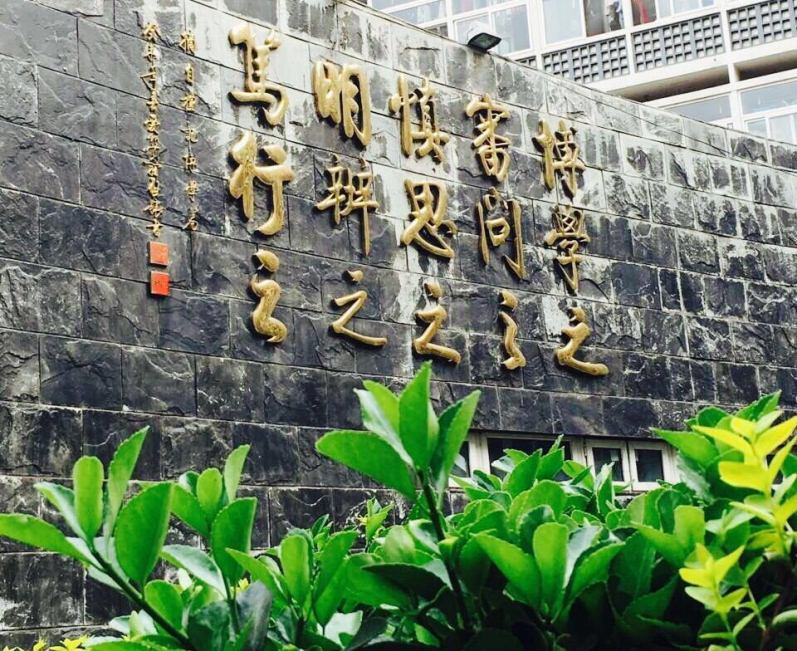
\includegraphics[width=\textheight]{pic/BJTU_Spring.jpg}
		\end{frame}
			
	\section{中端优化}

		\begin{frame}{SIMD 与多线程}
			手动实现一个多线程库
			
			\begin{itemize}
				\item \lstinline{__create_threads}:利用系统调用 \lstinline{sys_clone} 创建线程
				\item \lstinline{__join_threads}:利用系统调用 \lstinline{sys_exit} 和\lstinline{sys_waitid} 结束线程或等待线程结束
				\item \lstinline{__bind_core}:利用系统调用将线程绑定到 CPU 核心
				\item \lstinline{__lock}:互斥锁进入操作,用于修改已结束的线程数
				\item \lstinline{__unlock}:互斥锁退出操作,用于修改已结束的线程数
				\item \lstinline{__barrier}:barrier,用于线程间同步
			\end{itemize}
			
		\end{frame}
		
		\begin{frame}{SIMD 与多线程}
			\begin{itemize}
				\item 多线程:对于一个 $k$ 次迭代的循环,如果判断循环间无数据依赖,则将其分为 $\frac{k}{\mathrm{num\_threads}}$ 块并行执行
				\item SIMD:如果一个循环中没有分支,且每次循环间无数据依赖,且每条指令都能换成 SIMD 指令,且 SIMD 寄存器够用,则替换为 SIMD 指令
			\end{itemize}

		\end{frame}
	
	\section{后端优化}
	
		\begin{frame}{常规优化}
			\begin{itemize}
				\item Dead Code Elimination
				\item 对只含一条跳转指令的基本块,尽可能删除,但保证不出现基本块间的多重边
				\item 对只有一个前驱的基本块,将指令移动到前驱
				\item 分支指令转为条件执行
			\end{itemize}
		\end{frame}
		
		\begin{frame}{寄存器分配}
			\begin{itemize}
				\item 基于图染色问题的寄存器分配算法,优先保证生成代码的运行速度。
				\item 对 \lstinline{int} 和 \lstinline{float} 类型的伪寄存器分别执行寄存器分配。
				\item spill估价:优先spill保存常量的寄存器,优先spill使用频率较低的寄存器。
				spill策略考虑伪寄存器所在的循环深度\lstinline{depth} 与使用次数 \lstinline{cnt},计算$cnt * 4^{depth}$。
				\end{itemize}
		\end{frame}
	
\end{document}